\chapter{Seismic Noise} \label{chap2}
Seismic noise produces two types of problems for laser interferometric gravitational-wave detectors: it limits the low-frequency sensitivity and deteriorates the duty cycle. The former problem happens above 1 Hz and is associated with an anthropogenic activity. In order to reduce this human-induced seismic noise, constructing the detectors in the underground is an effective way because of far from human activity. On the other hand, the latter problem happens below 1 Hz and is generated by natural noise sources, such as the motion of the ocean, earthquakes, and earth tides. The underground environment, in contrast, cannot attenuate the lower-frequency seismic motions due to not local noises but global disturbances.

Regarding the low-frequency seismic noises, the property of the elastic waves on the ground, such as the common-mode rejection, effectively reduces the noises. The low-frequency elastic waves tend to shake the whole detector as a single object because the wavelength of the wave is several kilometers or more. Thus, the common-mode rejection effect appears in the small-scale GW detector such as LISM whose baseline is 20 m. For this reason, the LISM was able to operate stably due to the effect. However, this effect decreases in the large-scale baseline detectors, not only for current km-scale detectors but also for the planned Cosmic Explorer (CE) \cite{abbott2017exploring} and Einstein Telescope (ET) \cite{punturo2010einstein} whose baseline length is several ten km-scale. 

Section \cref{sec:31} offers a theoretical understanding of seismic noise as elastic waves. Section \cref{sec:32} describes some general properties of seismic noise. Finally, we discuss the problem in section \cref{sec:33}.

\section{Properties of seismic waves} \label{sec:31}
The ideal ground for GW detectors that must keep the optical cavity length constant is a {\it{rigid ground}} that does not stretch or contract the baseline length. The ground moves its center of mass without deformation when an external force is applied to the ground. In practice, however, the ground medium has elasticity and produces elastic waves when an external force is applied. The phase velocity of the elastic wave is finite. Thus a difference occurs in the displacement between two distant points. This becomes a baseline length fluctuation.

This section describes the baseline length fluctuation caused by elastic waves. We begin with the basic elastic waves in Section \cref{sec:311}. Section \cref{sec:312} discusses how elastic waves cause baseline length expansion and contraction for different length baselines, and shows that the longer baseline is more susceptible to the low-frequency seismic waves.

\begin{figure}[h]
  \begin{center}
    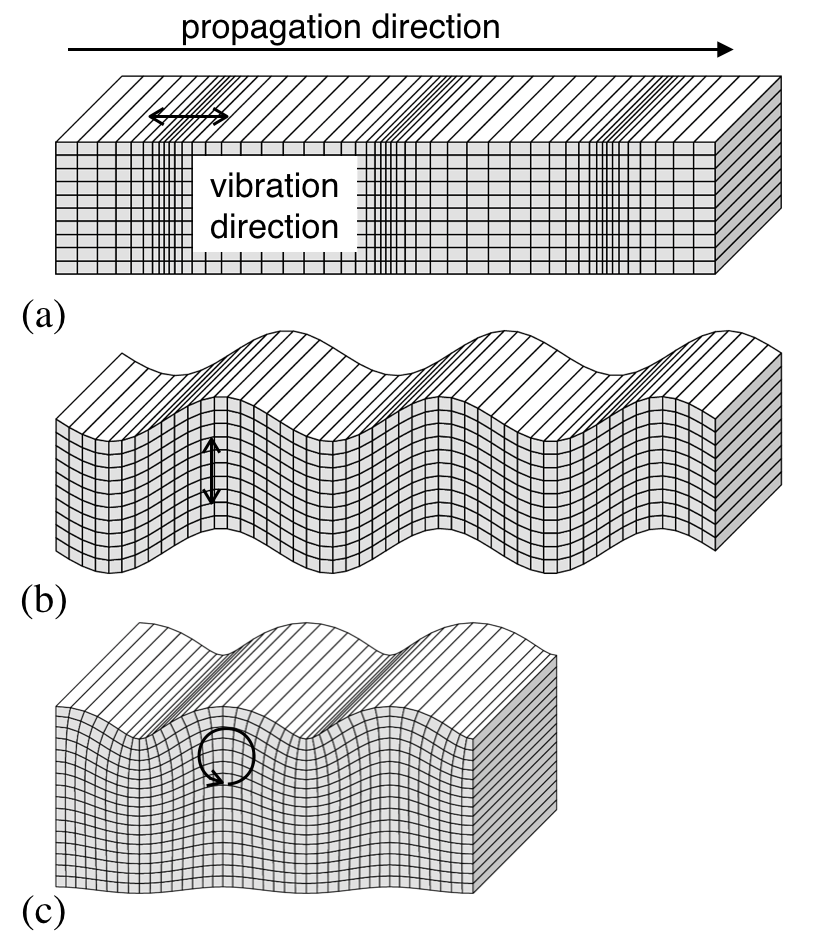
\includegraphics[width=9.0cm]{./img_chap3/img303.png}
    \caption{(a) longitudinal wave known as P-wave (b) transverse wave known as S-wave (c) Rayleigh wave \cite{shearer_2009}.
    }\label{img:img303}    
  \end{center}
\end{figure}


\subsection{Seismic Waves}\label{sec:311}
Seismic waves can be roughly categorized into body waves and surface waves. Body waves are the elastic waves propagating in a medium, and surface waves are the elastic waves propagating at a boundary between two different media. These elastic waves have different propagation methods and different phase velocities.

For simplicity, consider the seismic waves propagating in the homogeneous medium without external forces. The elastodynamic wave equation is given by 
\begin{eqnarray}\label{eq:eq_1}
  \rho{\bm{\ddot{u}}} = (\lambda+2\mu)\nabla(\nabla\cdot\bm{u}) - \mu\nabla\times(\nabla\times\bm{u}),
\end{eqnarray}
where $\bm{u}$ is the displacement field vetor of the medium, $\rho$ denotes density of the medium, and $\lambda,\,\mu$ are Lame's first and second parameter \cite{hasegawa2015jishin}.

\subsubsection{Body Waves}
From Eq.(\ref{eq:eq_1}), we can obtain two characteristic waves; longitudinal wave and transverse wave. Using Helmholtz's decomposition, we represent the displacement field vector $\bm{u}$ as
\begin{eqnarray} 
  \bm{u} &=& \nabla\phi + \nabla\times\bm{\psi}, \label{eq:eq_4}
\end{eqnarray}
where $\phi$ is the scalar potential, and $\bm{\psi}$ is the vector potential. The first term shows the seismic wave with changing the volume of the media, and the second term shows the seismic wave without changing that. Substitute Eq.(\ref{eq:eq_4}) into Eq.(\ref{eq:eq_1}) and after some vector algebra, one can obtain two wave equations;
\begin{eqnarray}
  \ddot{\phi} &=& v_{L}^2\nabla^2\phi \label{eq:eq_5},\\
  \ddot{\psi} &=& v_{T}^2\nabla^2\psi \label{eq:eq_6}, 
\end{eqnarray}
where $v_{L},\,v_{T}$ are defined as 
\begin{eqnarray}
  v_{L} = \sqrt{\frac{\lambda+2\mu}{\rho}},\
  v_{T} = \sqrt{\frac{\mu}{\rho}}. \label{eq:eq_7}
\end{eqnarray} 
Because the scalar potential and the vector potential are obey the wave equation Eq.(\ref{eq:eq_5}) and Eq.(\ref{eq:eq_6}) respectivly, the general solutions of these potentials are given as
\begin{eqnarray}
  \phi &=& \phi_{0}(\omega{t}-\bm{k}\cdot{\bm{x}}) \label{eq:eq_8}\\
  \bm{\psi} &=& \bm{\psi_{0}}(\omega{t}-\bm{k}\cdot{\bm{x}}) \label{eq:eq_9},
\end{eqnarray}
where $\omega,\,\bm{k}$ are the angular frequency and the wave vector, respectively. One can obtain the divergence component of the displacement filed vector $\bm{u}$ as
\begin{eqnarray}
  \bm{u}_{\mathrm{div}} = \nabla{\phi_{0}(\omega{t}-\bm{k}\cdot{\bm{x}})} =-\bm{k}{\phi}.
\end{eqnarray}
The displacement vector $\bm{u}_{\mathrm{div}}$ whose phase velocity is $v_{L}$ propagates along with direction of the wave vector. This means that $v_{L}$ is the phase velocity of a longitudinal wave. On the other hands, one can obtain the curl component of $\bm{u}$ as
\begin{eqnarray}
  \bm{u}_{\mathrm{rot}} = \nabla\times{\bm{\psi_{0}}(\omega{t}-\bm{k}\cdot{\bm{x}})} =-\bm{k}\times{\bm{\psi}}.
\end{eqnarray}
This displacement vector $\bm{u}_{\mathrm{rot}}$ whose phase velocity is $v_{T}$ is perpendicular to the wave vector. Thus, $v_{T}$ is the phase velocity of a transverse wave.

The phase velocity of the longitudinal wave $v_{L}$ is higher than that of the transverse wave $v_{T}$;
\begin{eqnarray}
  v_{L} > v_{T}.\label{eq:eq_10}
\end{eqnarray}
because $\lambda$ and $\mu$ are positive numbers. Therefore, the former wave is called primary wave (P-wave), and the latter wave is called secondary wave (S-wave) due to the time delay of arrival. Figure \ref{img:img303} shows the ground motion caused by P and S waves.


\subsubsection{Surface Wave (Rayleigh waves)}
If there is a free surface such as the ground surface, the surface wave propagates on the surface. Here, we particularly describe surface waves called Rayleigh waves. Figure \ref{img:img303} shows the ground motion caused by the Rayleigh wave. As shown in Figure \ref{img:img301}, consider a seismic wave propagating in the x-axis direction in a semi-infinite homogeneous medium. In this figure, P-wave and S-wave which are oscillating in the x-z plane exist. Assuming that these waves propagate at the same phase velocity $c_{R}$, the velocity can be expressed as a Rayleigh wave equation given as
\begin{eqnarray}\label{eq:eq_11}
\left(\frac{c_{R}^{2}}{c_{S}^{2}}\right)^{3}-8\left(\frac{c_{R}^{2}}{c_{S}^{2}}\right)^{2}+8\left(3-\frac{2}{\gamma^2}\right)\left(\frac{c_{R}^{2}}{c_{S}^{2}}\right)-16\left(1-\frac{1}{\gamma^2}\right)=0,
\end{eqnarray}
where $c_{\mathrm{S}}$ is the phase velocities of the S-wave, and $\gamma\equiv c_{\mathrm{P}}/c_{\mathrm{S}}$, where $c_{\mathrm{P}}$ is the phase velocity of the P-wave \cite{hasegawa2015jishin}. In the case that $0 < (\frac{c_{R}^2}{c_{S}^2}) <1$, the velocity has a physically meaningful value. We can calculate the phase velocity of the Rayleigh waves if the velocity of the both P-wave and S-wave. According to Eq.\ref{eq:eq_11}, the ratio $\frac{c_R}{c_S}$ is a function of the ratio $\gamma$. For example, because the phase velocity of P-wave and S-wave are $5.54\pm0.05\,\mathrm{km/s}$ and $3.05\pm0.06\,\mathrm{km/s}$, respectively, according to measurements in Kamioka mine \cite{takemoto2003}. Thus, the phase velocity of the Rayleigh wave almost $3\,\mathrm{km/s}$ in the Kamioka mine. 

\subsubsection{Depth dependence of the amplitude of the Rayleigh wave}
The displacement amplitude of the Rayleigh wave depends on the depth. Figure \ref{img:img302} shows the amplitude of the Rayleigh wave in the $x$ and $z$ directions ($u_x,\, u_z$) as a function of the depth $z'$ normalized by the wavelength of the Rayleigh wave \cite{hasegawa2015jishin}. From this figure, it can be seen that the $x$ component of the Rayleigh wave decreases at a depth of 1/4 wavelength. Therefore, the underground environment can reduce seismic noise caused by Rayleigh waves. In the underground environment, the horizontal motion of Rayleigh waves, which are surface waves, can be reduced, but P waves and S waves, which are body waves, cannot be reduced in such way.

The vibration component which is a problem for the gravitational wave detectors is the baseline length expansion and contraction represented by the differential component of the horizontal motion between two points. Fortunately, this component can be reduced.

\begin{figure}[h]
  \begin{minipage}[t]{0.5\hsize}
    \centering      
    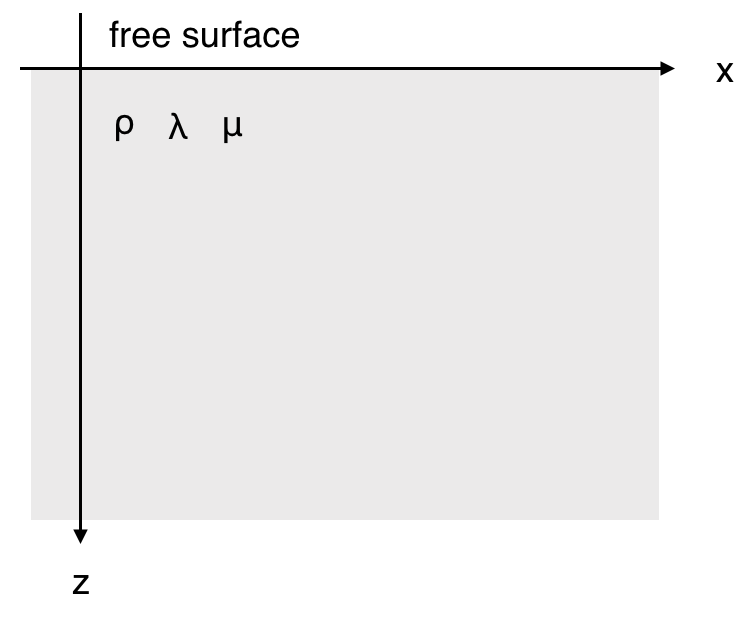
\includegraphics[width=9.0cm]{./img_chap3/img301.png}
    \caption{Semi-infinite medium. Where $z<0$, homogeneous medium fill the space with density $\rho$ and Lame's first and second parameter; $\lambda$ and $\mu$. Where $z=0$, there are free surface.}\label{img:img301}
  \end{minipage}    \hspace{1pt}    
  \begin{minipage}[t]{0.5\hsize}
    \centering
    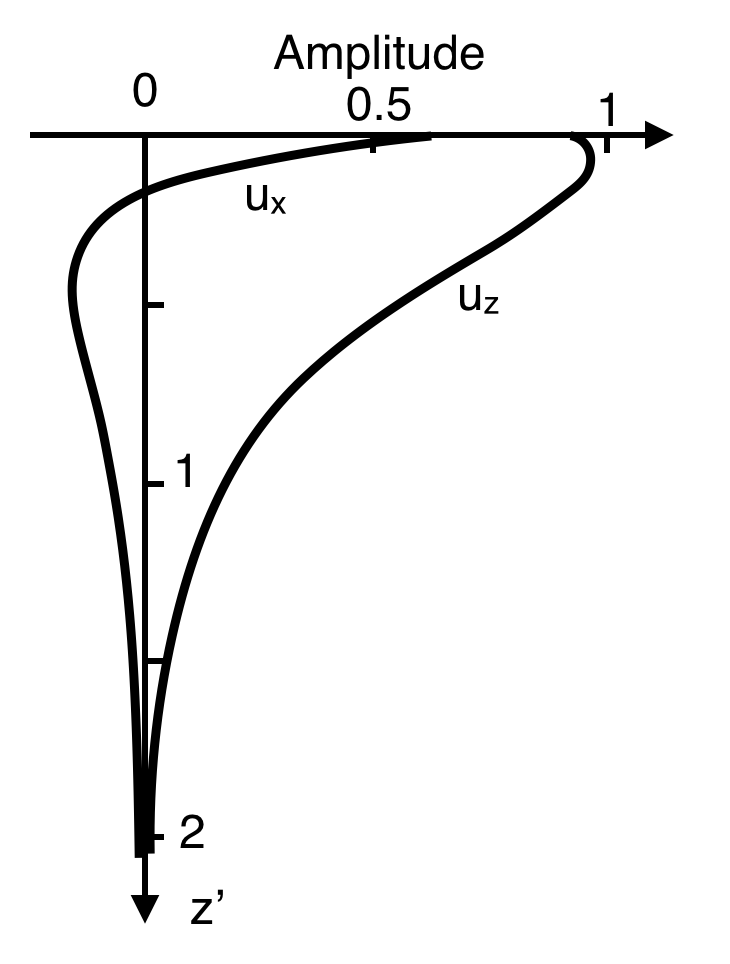
\includegraphics[width=6.0cm]{./img_chap3/img302.png}
    \caption{Depth dependance of the amplitude of the Rayleigh wave cited from \cite{hasegawa2015jishin}. $u_x$, $u_z$ are the amplitude of the Rayleigh wave which given by Eq.\label{eq:eq} in the case $\lambda=\mu$. $z'$ is the normalized depth given by $z'=z/(k/2\pi)$, where $z$ is the depth and $k$ is the wavevector of the Rayleigh waves.}\label{img:img302}
  \end{minipage}
\end{figure}



\subsection{Common Mode Rejection of the Baseline} \label{sec:312}
The low-frequency seismic motion having a long wavelength is easy to move two distant points in the same phase, so that the variation of the baseline length, which is the opposite phase, is reduced. In this subsection, such a common mode rejection effect is discussed by assuming that the seismic wave is a plane wave.

Consider the motion of the ground whose displacement is given by the displacement field $\bm{u}(t,\,\bm{x})$, where $t$ is time and $\bm{x}$ is the position vector.

\begin{figure}[h]
  \begin{center}
    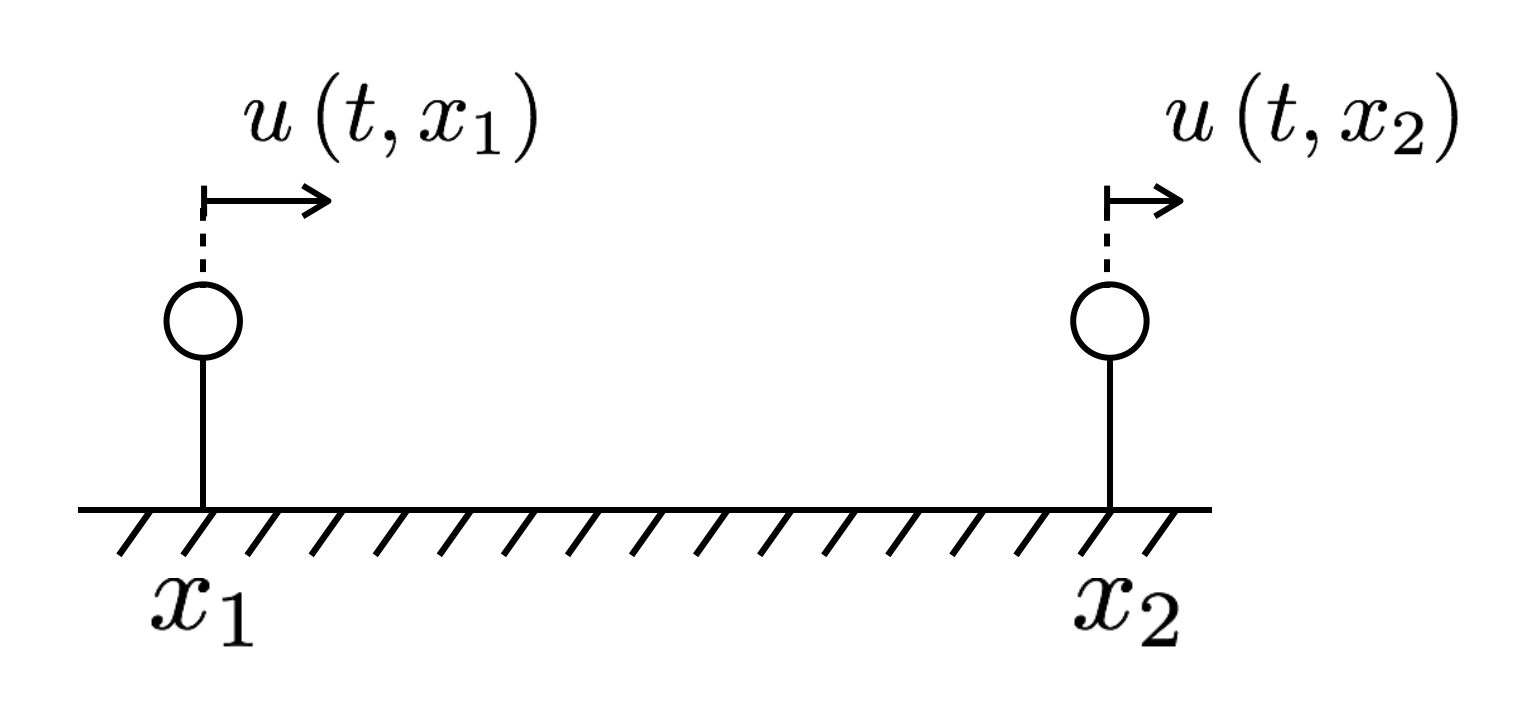
\includegraphics[width=9.0cm]{./img_chap3/img315.png}
    \caption{The two points are sparated by a distance L along the X axis. $\bm{u}(t,\bm{x})$ is the displacement field vector, where $t$ denotes the time and $\bm{x}$ denotes the location vector.}\label{img:img310}    
  \end{center}
\end{figure}

\subsubsection{Differential Motion and Common Motion}
We define the motion of two points shown in Figure (\ref{img:img310}) as $\bm{u}_1=\bm{u}(t,\bm{x}_1)$ and $\bm{u}_2=\bm{u}(t,\bm{x}_2)$, respectively, where $x_1$ and $x_2$ are the position vector of each points. The motion of the two points can alternatively be represented as the differential motion and the common motion defined as
\begin{eqnarray}
  \bm{u}_{\mathrm{diff}} \equiv \frac{\bm{u}_{1}-\bm{u}_{2}}{\sqrt{2}}, \, \\ \label{eq:eq22}
  \bm{u}_{\mathrm{comm}}  \equiv \frac{\bm{u}_{1}+\bm{u}_{2}}{\sqrt{2}}. \label{eq:eq100}
\end{eqnarray}
These two components are normalized by $\sqrt{2}$ to conserve the total power.



\subsubsection{Common and Differential Motion Ratio (CDMR)}\label{sec:sec313}
To discuss the common-mode rejection effect, we define the power ratio of the common motion over the differential motion as common and differential motion ratio (CDMR). The power spectrum density (PSD) of CDMR is given by
\begin{equation}
  \mathrm{CDMR} \equiv \sqrt{\frac{\mathrm{Common\,Motion}}{\mathrm{Differential\,Motion}}} = \sqrt{\frac{P_{\mathrm{comm}}(\omega)}{P_{\mathrm{diff}}(\omega)}} \label{eq:eq23}
\end{equation}
where $P_{\mathrm{comm}},P_{\mathrm{diff}}$ are the PSDs of the differential and common motions, respectively. This ratio is useful to describe how the differential motion is reduced in the baseline compared to the common motion.

To obtain these PSDs, we convert from the autocorrelation function of these. Therefore, autocorrelation function $C_{\mathrm{diff}}$ of the differential motion is given by its definition in Eq.(\ref{eq:eq22})
\begin{eqnarray}
  C_{\mathrm{diff}}(\tau) &=& \frac{1}{2}
  \biggl\langle
  \biggl[ u_{1}(t)-u_{2}(t) \biggr] \biggl[ u_{1}(t+\tau)-u_{2}(t+\tau) \biggr]
  \biggr\rangle \\
  &=& \frac{1}{2}\biggl[ C_{11}(\tau) - C_{12}(\tau) - C_{21}(\tau) + C_{22}(\tau) \biggr], 
\end{eqnarray}
where $C_{ij}$ are the autocorrelation functions of each point and defined as $ C_{ij} \equiv \langle u_{i}(t)u_{j}(t+\tau)\rangle,\, (i=1,2,\,j=1,2)$. Here, one can obtain the power spectrum density of differential motion $P_{\mathrm{diff}}(\omega)$ as 
\begin{eqnarray}
  P_{\mathrm{diff}}(\omega) &=& \frac{1}{2}\biggl[ P_{1}(\omega) + P_{2}(\omega) - P_{12}(\omega) - P_{12}^*(\omega) \biggr]\\
  &=& \frac{1}{2} \biggl[ P_{1}+P_{2} - \mathrm{Re}\left[\mathrm{coh} \right]\times2\sqrt{P_{1}P_{2}} \biggr], \label{eq:eq31}
\end{eqnarray}
where $P_{1}(\omega),P_{2}(\omega)$ are the PSDs of each points, and $P_{12}(\omega)$ are the cross spectrum between the two points. The parameter $\mathrm{coh}$ is the complex coherence between them defined by
\begin{eqnarray}
  \mathrm{coh} \equiv \frac{P_{12}}{\sqrt{P_{1}P_{2}}}.
\end{eqnarray}
Furthermore, assuming that seismic wave propagating each points does not decay, which means $P_{1}=P_{2} \equiv P$, one can compute the $P_{\mathrm{diff}}(\omega)$ as 
\begin{eqnarray} \label{eq:eq32}
  P_{\mathrm{diff}}(\omega) = P (1-\mathrm{Re}\left[\mathrm{coh}\right]).
\end{eqnarray}
Similarly, the PSD of the common motion can be calculated as
\begin{eqnarray}
  P_{\mathrm{comm}}(\omega) = P (1+\mathrm{Re}\left[\mathrm{coh}\right]).
\end{eqnarray}
Finaly, the PSDs of the CDMR defined Eq.(\ref{eq:eq23}) in the case that the seismic wave is plane wave is represented as
\begin{eqnarray}
 \mathrm{CDMR} = \sqrt{\frac{1 + \mathrm{Re} \left[\mathrm{coh} \right] }{1 - \mathrm{Re} \left[\mathrm{coh} \right]}}\,. \label{eq:eq33}
\end{eqnarray}
Eq.(\ref{eq:eq33}) indicates that CDMR can be expressed by only the coherence $\mathrm{coh}$ between of two points. For example, CDMR tends to be larger when $\mathrm{coh}$ close to 1. This means that the differential motion is less than the common motion because the two points move together in the same direction. This means that the common mode rejection effect.

\subsubsection{Uniform Plane Wave Model}
\begin{figure}[h]
  \begin{center}
    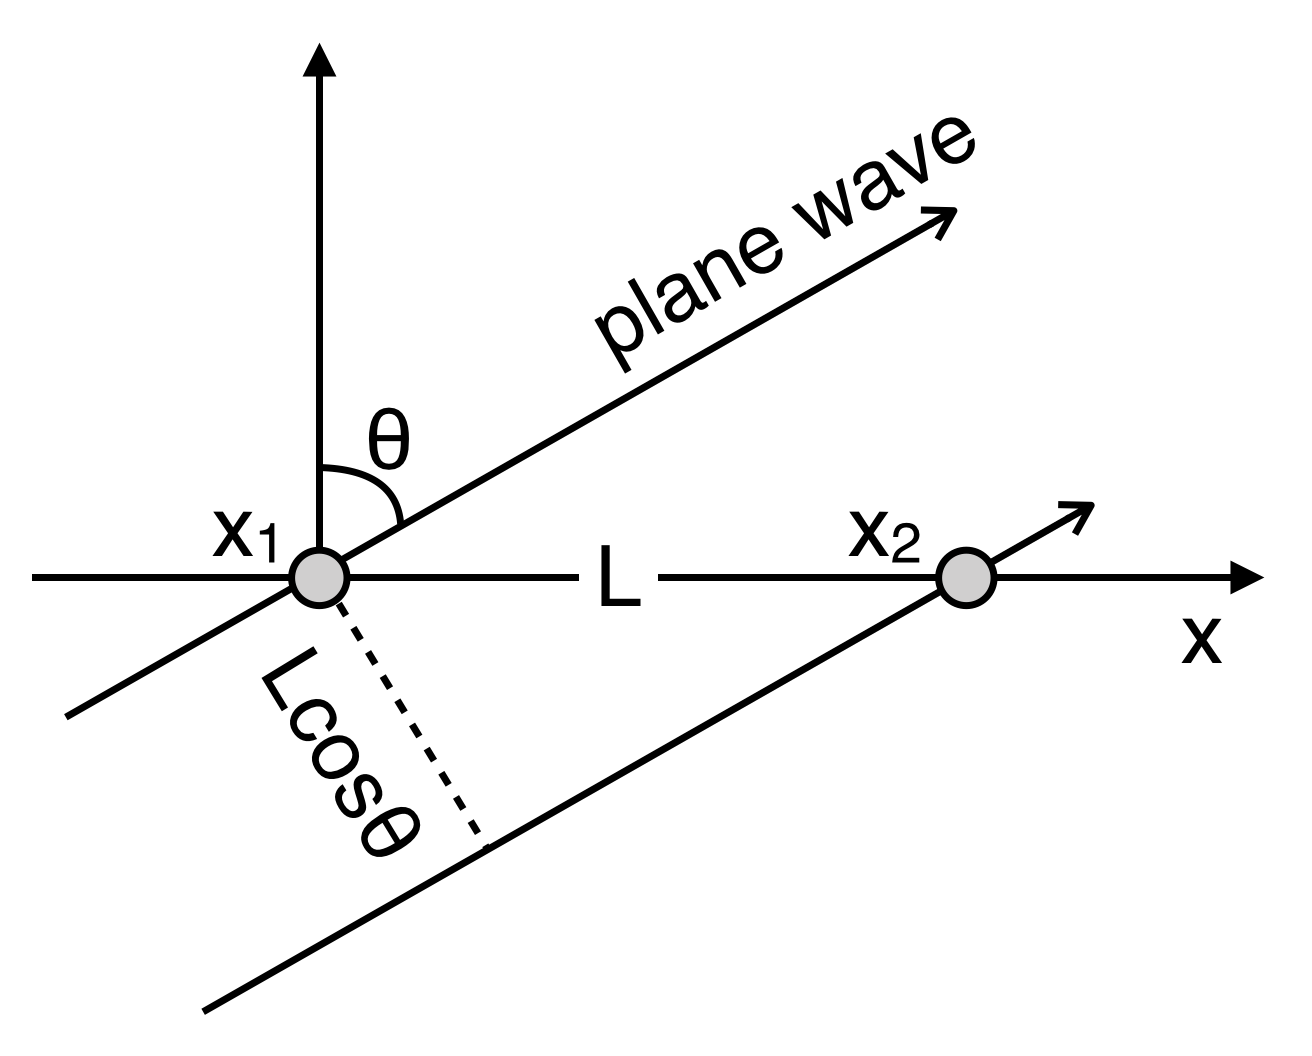
\includegraphics[width=6.0cm]{./img_chap3/img304.png}
    \caption{Single plane wave passing through two points with azimuth angle $\theta$. Top view of Figure {\ref{img:img310}}.}\label{img:img304}
  \end{center}
\end{figure}

Consider the PSD of the CDMR when the plane waves are distributed uniformly around the azimuth. This case is true when the seismic noise sources are distributed uniformly. The coherence in the case that the single plane wave propagating with the azimuth angle $\theta$ along the direction of the x-axis in Figure (\ref{img:img304}) is given by
\begin{equation}
  \mathrm{coh} = \exp\left[{i\frac{L\mathrm{cos}\theta\omega}{c}}\right], \label{eq:eq18}
\end{equation}
where $L$ is the distance between the two points.

The coherence in case that the plane waves propagates uniformly is given by the integral of Eq.(\ref{eq:eq18}) overall direction;
\begin{eqnarray} \label{eq:eq19}
  \mathrm{coh} &=& \frac{1}{2\pi} \int_{-\pi}^{\pi} e^{i\frac{\omega}{c} L\cos \theta} d \theta = J_0\left(\frac{L\omega}{c}\right).
\end{eqnarray}
where the coherence is normized azimuth angle. Therefore, the PSD of the CDMR is given as
\begin{equation}  \label{eq:eq20}
  \mathrm{CDMR} = \sqrt{\frac{1+J_0(\frac{L\omega}{c})}{1-J_0(\frac{L\omega}{c})}} .
\end{equation}

\subsubsection{Comparison with different baseline length}
We show how the effect of common-mode rejection differs from the baseline length. The CDMR comparison with LISM, CLIO, KAGRA is shown in Figure \ref{img:img301}. We assume that the uniform plane wave model with the phase velocity of $3\,\mathrm{km/s}$, which means the uniform Rayleigh waves in the Kamioka mine. One can find that KAGRA which is the km-scale detector has few CDMR below $0.1\,\mathrm{Hz}$ than the other short-scale detectors. This means that the effect of the common-mode rejection is reduced on the long baseline. Thus, the ground vibration below 1 Hz is more significant than on the short baseline. 

\begin{figure}[h]
  \begin{center}
    \centering
    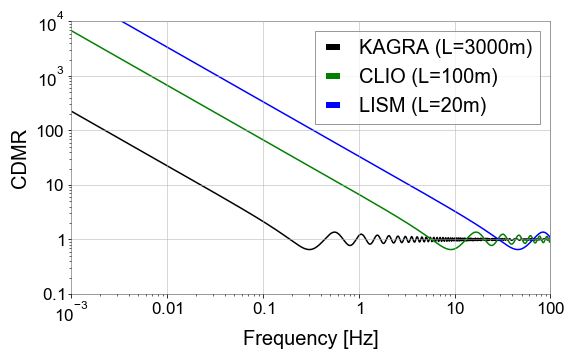
\includegraphics[width=12cm]{./img_chap3/img329.png}
    \caption{CDMR given in Eq.(\ref{eq:eq20}), of the underground GW detectors assuming the uniform plane waves model with phase velocity of 3 km/s. Black is the CDMR of KAGRA with the 3000 m baseline, green is the CDMR of CLIO with the 100 m baseline, and blue is the CDMR of LISM with the 20 m baseline.}\label{img:img301}
    \centering      
    %% 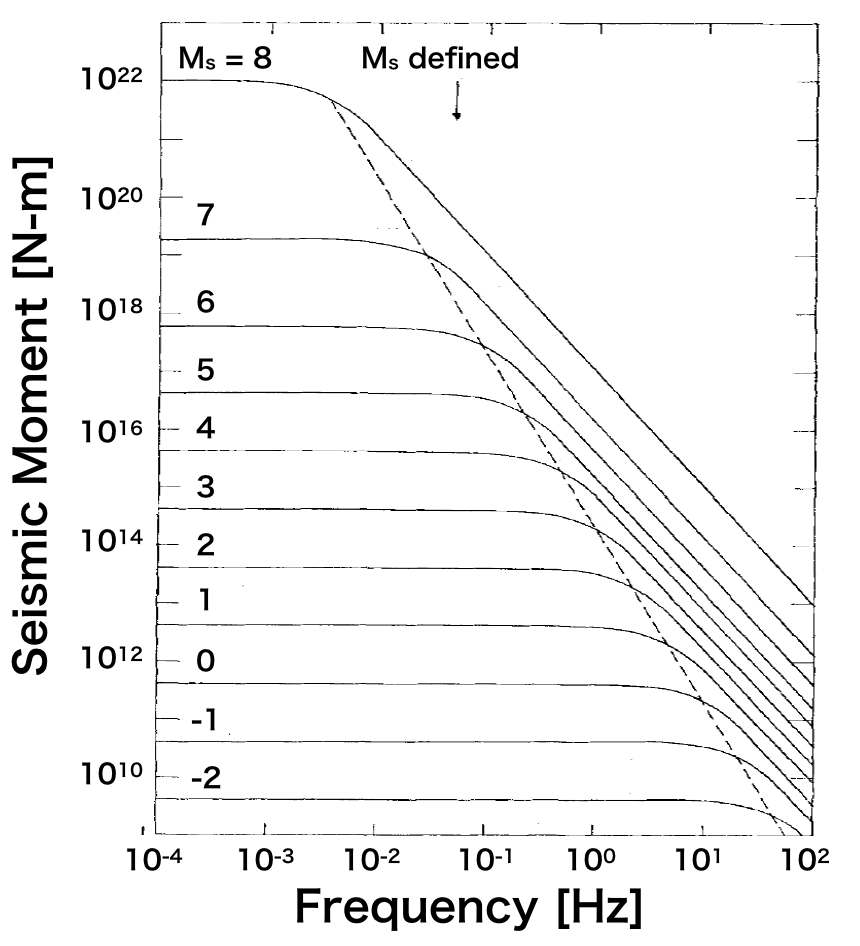
\includegraphics[width=12cm]{./img_chap3/img328.png}
    %% \caption[The power ratio of the differential motion of the baseline over the motion at single point; $P_{\mathrm{diff}}/P$ of Eq.(\ref{eq:eq21})]{The power ratio of the differential motion of the baseline over the motion at single point; $P_{\mathrm{diff}}/P$ of Eq.(\ref{eq:eq21}). This ratio gives the estimation of the PSD of baseline length fluctuation from the }\label{img:img302}
  \end{center}
\end{figure}


\newpage
\section{Seismic Noise}\label{sec:32}
In this section, we introduce the noise source of the seismic motion. Characteristics of the seismic noise are related to its origin spatially and temporally. The noise sources are spread anywhere; footsteps, traffic, ocean waves, and these amplitude depends on day-night or weather condition.

As summarized in Table \ref{tb:31}, the seismic noises above $1\,\mathrm{Hz}$ are clearly correlated with cultural activities, and that below this frequency are excited by the natural phenomena \cite{bonnefoy2006nature}.
\begin{table}[h] 
  \begin{center}
    \caption{Two types of seismic noise}\label{tb:31}
    \begin{tabular}{lll} 
      \hline      
      Type of noise & Frequency Band & Sources \\ \hline \hline
      Cultural Noise & $> 1\,\mathrm{Hz}$ & traffic, machinaries, foot steps\\
      Natural Noise  & $< 1\,\mathrm{Hz}$ & ocean, air pressure, earth tides\\
    \end{tabular}
  \end{center}
\end{table}

This boundary frequency between cultural or natural depends on the soil structure. At the sediment site such as the LIGO \cite{Daw_2004} and Virgo site \cite{Beker_2012}, the cultural noise can be shifted to a lower frequency and appear below $1\,\mathrm{Hz}$. On the other hand, at the hard rock site such as the KAGRA site, the cultural noise can be distinguished from the natural noise for its diurnal variability and apparent only above $1\,\mathrm{Hz}$.


\subsection{Cultural Noises} \label{sec:321}
The cultural seismic noise contaminates the sensitivity of gravitational-wave detectors in the frequency range of interest for gravitational-waves sources, above $1\,\mathrm{Hz}$. In this frequency band, cultural noise is dominated by human activities. For example, seismic noise from traffic near the detectors is reported at the LIGO site \cite{schofield2000source}.
%and noise from the vibrations of building excited by winds is reported at Virgo site \cite{acernese2004properties}. 

\subsection{Natural Noises} \label{sec:322}
The natural seismic noise affects the stability of the GW detectors below $1\,\mathrm{Hz}$. These natural noises depend on the location. Figure \ref{img:img324} shows the noise spectra of the seismic noise measured by Peterson in 75 stations in the world \cite{peterson1993observations}. The new high noise model (NHNM) is a spectrum of the average of high background noise power in the stations. The primary contributions to the NHNM are coastal stations and inland stations on the soft soil. On the other hand, the new low noise model (NLNM) represents the seismic noise when microseismic is quiet. Especially, below 0.1 Hz, it represents the global seismic noise floor \cite{nishida2002origin}. 

\begin{figure}[p]
  \begin{center}   
    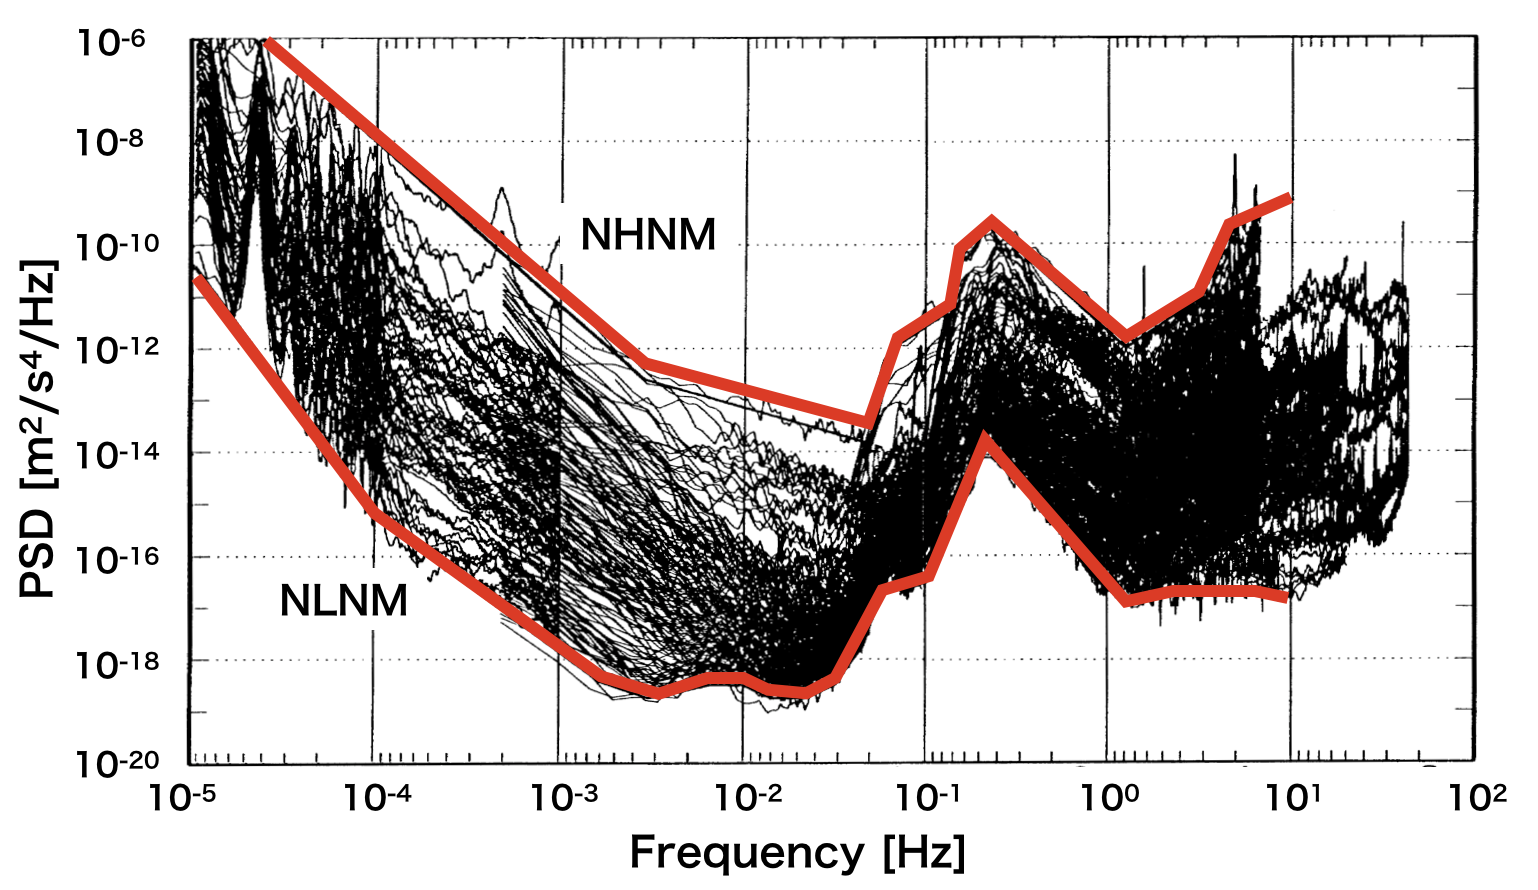
\includegraphics[width=12.5cm]{./img_chap3/img324.png}
    \caption{PSDs of the seismic noise obtained by Peterson in 75 stations in the world \cite{peterson1993observations}. Each of the black solid lines are PSDs divided into 5 different frequency band at the each stations. Each red lines are the new high noise model (NHNM) and the new low noise model (NLNM), respectively.}\label{img:img324}
  \end{center}
  \begin{center}   
    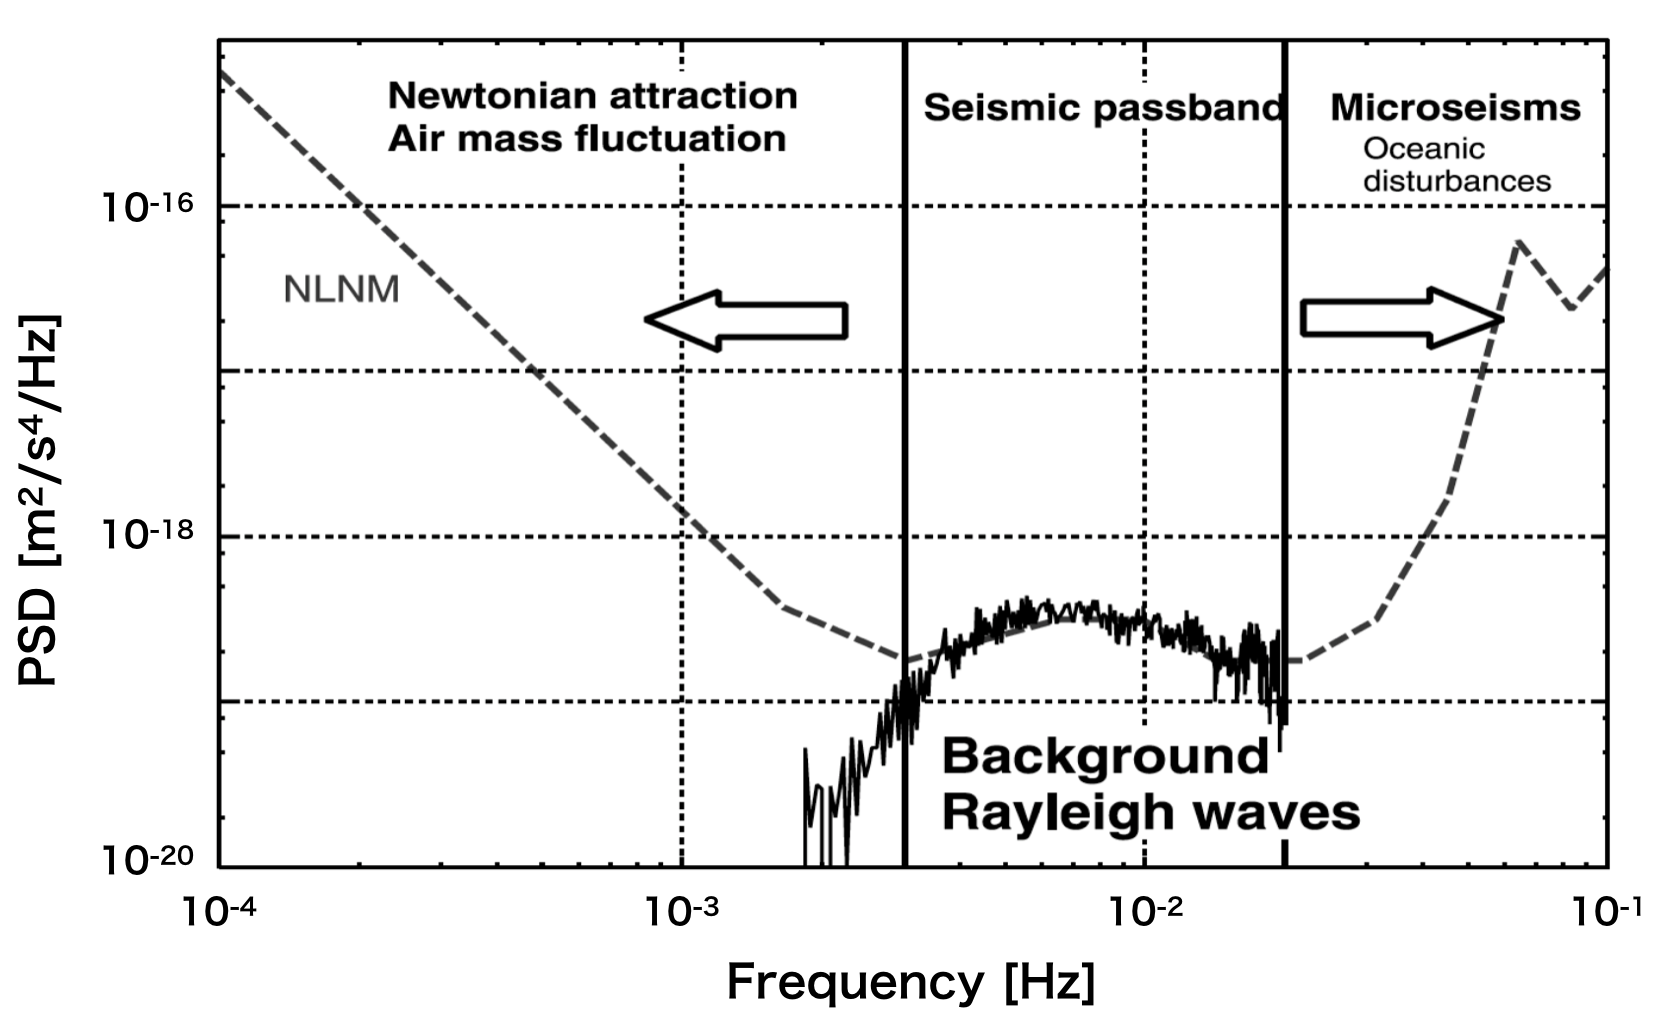
\includegraphics[width=13cm]{./img_chap3/img325.png}
    \caption{Noise contribution below $100\,\mathrm{mHz}$ \cite{nishida2002origin}. }\label{img:img325}
  \end{center} 
\end{figure}


\subsubsection{Microseisms}
Microseisms whose power peaked in the frequency range of $50$ -- $200\,\mathrm{mHz}$ are excited by oceanic waves. These seismic waves can be categorized by generating mechanism \cite{Bormann2012new}. The primary ocean microseisms are produced only in shallow waters in coastal regions. In these regions, the water wave energy can be converted directly into seismic energy either through vertical water pressure variations or by the impacts of the surf on the shores. Thus, there is a correlation between this microseismic peak and the swell at the beaches was known from the data sets studied by \cite{haubrich1963comparative}. The secondary ocean microseisms could be explained by the superposition of ocean waves of equal period traveling in opposite directions. Therefore, generating standing gravity waves of half the period \cite{longuet1950theory}.

%% The RMS amplitude spectra of both types of microseisms are strongly dependent on the low pressure on the ocean \cite{naticchioni2014microseismic}. ({\color{red}{論文の内容で補足する}})

\subsubsection{Seismic Noise Below $20\,\mathrm{mHz}$}
Below the microseismic band, the main seismic noise source is an atmospheric pressure change; Rayleigh waves excited by air fluctuation on the surface, and the deformation of the Earth's crust caused by the Newtonian attraction of air mass fluctuation \cite{sorrells1971earth,zurn1995noise}. Figure \ref{img:img325} shows PSDs of the NLNM and the seismic motion excited by the Rayleigh waves \cite{nishida2002origin}. The noises caused by Rayleigh waves are consistent with the NLNM between $2\,\mathrm{Hz}$ and $30\,\mathrm{mHz}$. The noises caused by the Newtonian attraction are increased PSD increases rapidly with decreasing frequency below two mHz.

Although Seismic motion in this band is usually quiet, large earthquakes often excite the ground in this band \cite{aki2002quantitative,aki1967scaling}.

%% Although the seismic noise depends on both the fault and propagation path, here, we assume the same fault. In this situation, it is known that the measurement can be explained by the model (omega-square model);
%% \begin{eqnarray}
%%   s(\omega) = \displaystyle\frac{S_0}{1+({\omega}/{\omega_0})^2}, \label{eq:eq_}
%% \end{eqnarray}
%% where $M_{\mathrm{s}}$ is the surface magnitude \cite{gutenberg1945study}, $S_0$ is a constant propotional to $M_{\mathrm{s}}$, $\omega_0$ is the corner frequency propotional to $(M_{\mathrm{s}})^{1/3}$. The spectral of Eq.(\ref{eq:eq_})with several surface magnitude are ploted in Figure \ref{img:img328}. One can find that the large earthquakes tend to excite the ground at lower frequency.


\subsubsection{Earth tides}
At even lower frequencies, the earth deformed by tidal forces due to the attraction of Sun and Moon in diurnal and semi-diurnal periods \cite{agnew2005earth}. 

%% \begin{figure}[h]
%%   \begin{center}   
%%     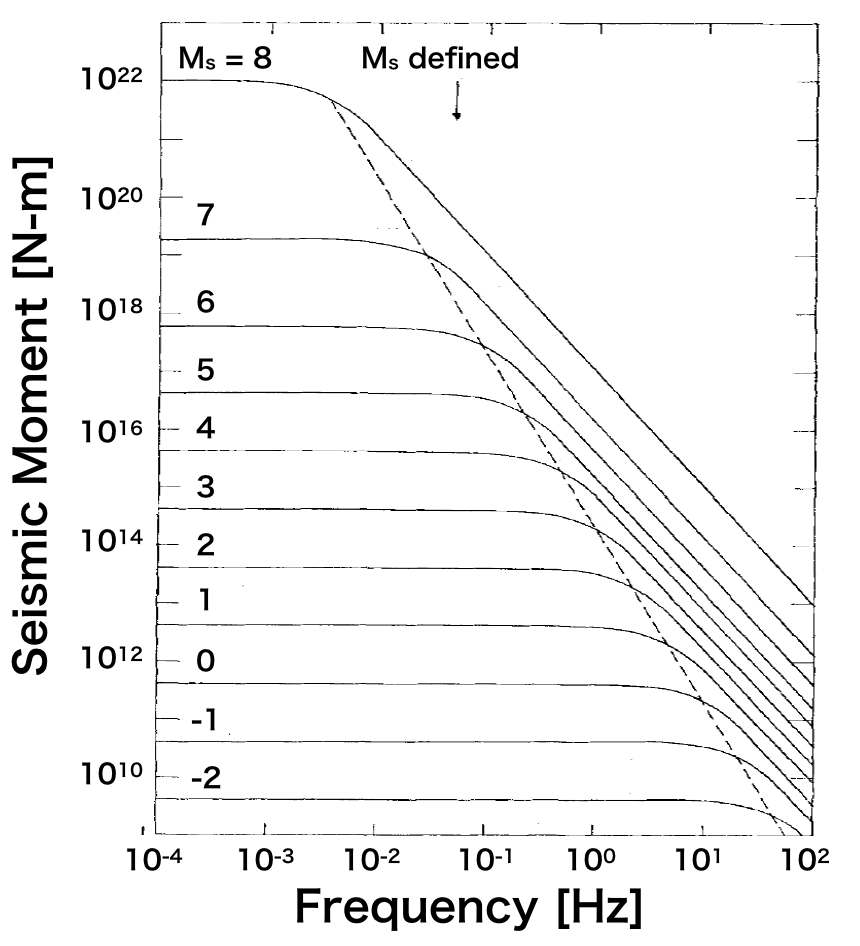
\includegraphics[width=8cm]{./img_chap3/img328.png}
%%     \caption{omega-square model \cite{aki1967scaling}}\label{img:img328}
%%   \end{center}
%% \end{figure}


\newpage
\section{Seismic Noise in the KAGRA Mine} \label{sec:33}
In this section, we characterized the seismic noise in the KAGRA site by using a seismometer installed at the site. Section \ref{sec:331} described the seismometer and signal acquisition system. Section \ref{sec:332} compared the seismic noise in KAGRA with the typical noise in the world. Section \ref{sec:333}, we discuss the common-mode rejection effect observed in the X and Y arms in KAGRA comparing with a simple model.

\subsection{Experimental Arrangement}\label{sec:331}
\begin{figure}[h]
  \begin{center}   
    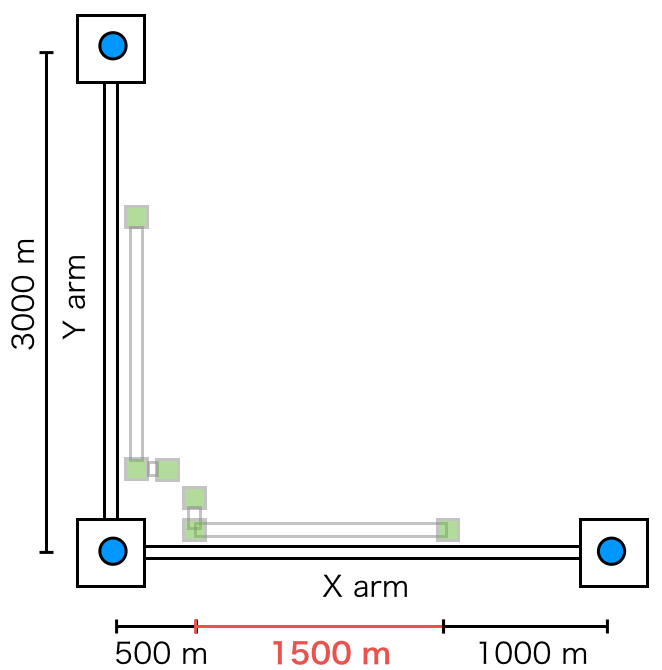
\includegraphics[width=8cm]{./img_chap3/img328a.png}
    \caption{Location of the seismometers (blue). KAGRA has three stations which are separated with 3 km; X-end, Y-end, and corner stations.}\label{img:img328a}
  \end{center}
\end{figure}

\subsubsection{Seismometers Array}
The Trillium 120-QA which is a three-axis, very broadband, and low-noise seismometer, is used. These three outputs are proportional to the ground velocity of two horizontal and one vertical, respectively. 

\begin{figure}[h]
  \begin{center}   
    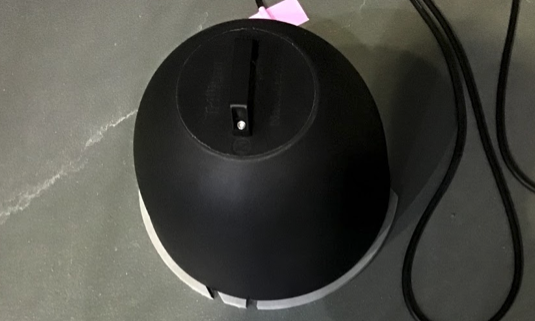
\includegraphics[width=9.0cm]{./img_chap3/img316.png}
    \caption{Trillium 120-QA installed on the second floor at X-end area, which is coverd by black thermal insulation cover}\label{img:img316}
  \end{center}
\end{figure}

The seismometer is housed in the black thermal insulation cover, as shown in Figure \ref{img:img316}. Thermal insulation protects two broad categories of thermal couplings that can cause unwanted noise \cite{trillium120manual}. First is the direct coupling to the sensitivity. This coupling typically increases the noise of the vertical channel as a periodic diurnal variation caused by the day-to-night temperature cycle, because the springs that suspended the inertial masses are temperature sensitive. The second is the coupling to tilt from the thermal fluctuation. Tilt converts the vertical acceleration of gravity into horizontal acceleration. This thermally induced tilt noise on the horizontal will be larger than the direct thermal coupling on the vertical channel. To be low sensitivity to both tilt and temperature, this model has a function to center the inertial mass after the initial installation.

The signals of the seismometer are recorded through the data acquisition system developed by LIGO \cite{bork2001overview}. The analog signal is converted to a digital signal by the 16-bit analog-to-digital converters (ADC) with 16384 $\mathrm{Hz}$ sampling. This analog signal is amplified with 30 dB so that the ADC noise does not mask this signal. 

\subsubsection{Data Processing}
The estimation of the amplitude spectrum densities is calculated by the average of 32 segments with 50\% overlapping. The single segment has $256\, (2^8)\,\mathrm{sec}$. The FFT calculation of each segment is done after detrending the linear trend and multiplying the Hanning window. 

The error bars of this spectral is calculated by chi-square distribution. For example, the spectrum averaged by 32 obeys the chi-square distribution with 32 degrees of freedom. The confidence interval of $100(1-\alpha)\,\%$ with degrees of freedom $\nu$ is given by 
\begin{eqnarray}
  \frac{\nu{\hat{G}(f)}}{\chi^2(\nu,1-\frac{\alpha}{2})} \leq G(f) \leq \frac{\nu{\hat{G}(f)}}{\chi^2(\nu,\frac{\alpha}{2})},
\end{eqnarray}
where $f$ is the frequency and $\hat{G}(f)$ is estimator of spectrum. Therefore, the confidence level of 95\% is 
\begin{eqnarray}
  \nu/\chi^2(\nu,1-\frac{\alpha}{2}) \leq G(f)/\hat{G}(f) \leq \nu/\chi^2(\nu,\frac{\alpha}{2}).
\end{eqnarray}
In case that degrees of freedom is 32, the spectral point lies within 0.65 to 1.75 of the estimates.

\subsection{Study of Long-term Seismic Noise} \label{sec:332}
It is known from the measurement by Peterson that the seismic noise varies from place to place.  In this subsection, we compared the stationary seismic noise of KAGRA obtained in one year with Peterson's measurements. 

Long-term seismic noise is measured by a seismometer installed on the second floor of the X-end station. This area is placed 200 $\mathrm{m}$ underground from the surface of the mountain. In comparison to the corner area, human activity in the end area is less because the corner area has parking lots. In comparison to the Y-end area, there is no entrance connected to other mines. Therefore, the X-end area is relatively quiet in the KAGRA mine, regarding the seismic noise induced by human activity. 

We estimated the noise spectral using the one-year data, which does not include the glitch noises such as the earthquake or circuit noise. Figure \ref{img:img313} shows the amplitude spectral densities (ASDs) of the horizontal and vertical components of the acceleration. Below $40\,\mathrm{mHz}$, the horizontal noise is much larger than the vertical noise due to noise arise by temperature fluctuation, and the ten percentile of vertical noise is close to Peterson's NLNM estimation. This means that the KAGRA mine is also quiet with respect to anthropogenic noise enough to measure the background seismic noise floor in this band. From $40\,\mathrm{mHz}$ to $1\,\mathrm{Hz}$, in the microseismic noise band, the ten percentile of both components are middle of the NHNM and NLNM. This indicates that the microseismic in KARGA is not quieter than that in the inland station because the KAGRA site is located on $40\,\mathrm{km}$ far from Toyama bay. Above $1\,\mathrm{Hz}$, both components are close to the NLNM due to the underground environment.

In the environment of KAGRA, human-induced seismic noise above 1 Hz is quiet and approaches NLNM, but the seismic noise in the microseismic noise band is located in the middle of NHNM and NLNM. Thus, the effect of microseismic noise is not small, even in the underground.


\begin{figure}[h]
  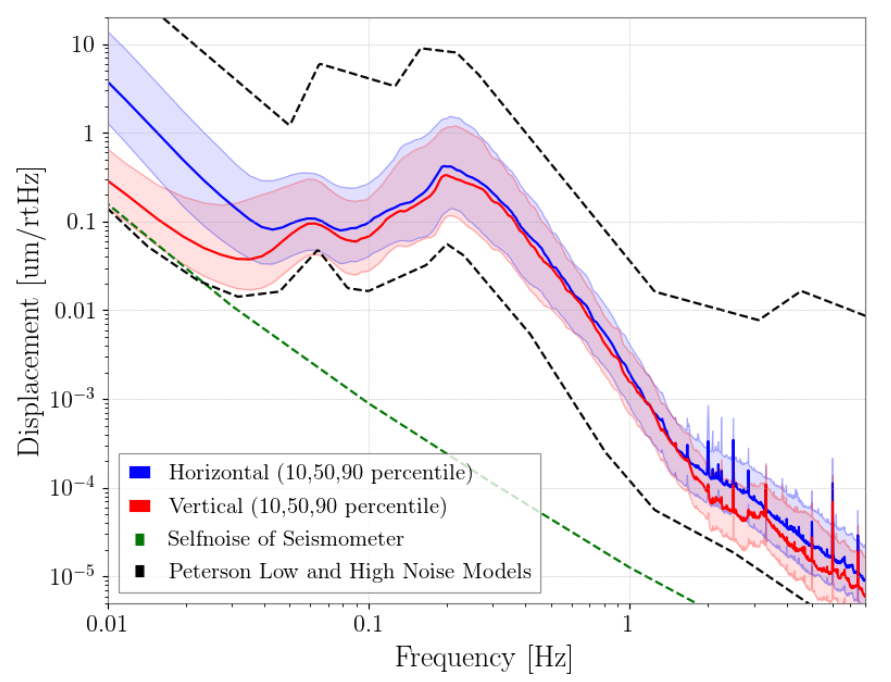
\includegraphics[width=13.0cm]{./img_chap3/img313.png}
  \caption{ The seismic noise in KAGRA mine. Red and blue are the amplitude spectral densities (ASDs) of horizontal and vertical components of the ground motion, respectively. Each component are shown by the 90, 50, 10 percentile of their ASDs, in order from top to bottom.}\label{img:img313}
\end{figure}

\subsection{Study of the Common Mode Rejection} \label{sec:333}
We have evaluated the common-mode rejection effect for the 3 km arms of KAGRA. For that purpose, we calculated the CDMR given by Eq.(\ref{eq:eq23}), using two seismometers pairs; the X-end and corner stations, and the Y-end and corner stations in Figure \ref{img:img328a}. For example, the differential (solid line) and common motion (dashed line) of the X-arm are calculated by the X-axis of each seismometer signal, which is proportional to the ground velocity. 

The top of Figure \ref{img:img319} shows the common and differential motion of the ground velocity. In this figure, ASDs of the velocity of the differential (solid line) and the common motion (dashed line) are shown. The red and blue indicate the motions of X-arm and Y-arm, respectively. As a reference, the black dashed line shows the self-noise of the Trillium 120Q broadband seismometer multiplied $\sqrt{2}$. Below 0.05 Hz, the ASDs are limited by the thermally induced tilt noise which is mentioned in section \cref{sec:331}. 

\begin{figure}[h]
    \begin{center}   
      
\includegraphics[width=13.0cm]{./img_chap3/img319.png}
      \caption{Comparison with the measured CDMR and the CDMR assumed the uniform plane waves model.}\label{img:img319}
    \end{center}
\end{figure}

The bottom of Figure \ref{img:img319} shows the comparison of the measured CDMR and the CDMR assumed a uniform plane wave model. The measured CDMR is given as red and blue solid lines whose colors indicate the X-arm and Y-arm, respectively. As a reference, the gray line indicates the CDMR assuming the uniform plane waves model in case the phase velocity is in the region from $5 - 3\,\mathrm{km/sec}$, and green dashed line is the CDMR assuming the no correlation between each endpoint of the baseline. The measured CDMR is consistent with the uniform model in $0.05 - 0.5\,\mathrm{Hz}$. Below this band, the CDMR is close to the no correlation model due to the noise of the seismometers. Below and above this band, the measured CDMR is consistent with the no correlation model.


%% \section{Summary of the Chapter}
%% ({\color{red}{もっと的確にまとめる}})
